\documentclass[10pt,aspectratio=169,english,fontset=none]{beamer}
% \overfullrule=1pt
\usepackage[fontset=windows]{ctex}
% \usepackage[charter]{mathdesign}
\usepackage{hologo}
\usepackage{luamesh}

\usepackage{babel}
\usepackage{pgfpages}
\usepackage{tcolorbox}
\usepackage{biblatex}
%\hypersetup{colorlinks=true}

\tcbuselibrary{listings,breakable}
\tcbuselibrary{documentation}
\tcbset{
    color command=AmurmapleRed,
    color environment=AmurmapleRed,
    color option=AmurmapleGreen
}
\usetheme[
%nogauge,
nomail,
delaunay,
%amurmapleblue
]{Amurmaple}

\lstset{
  numberstyle=\footnotesize\color{gray},
  keywordstyle=\ttfamily\bfseries\color{structure},
  basicstyle=\ttfamily\normalsize,
  commentstyle=\itshape\color{gray},
  stringstyle=\ttfamily,
  showstringspaces=false,
  language=[LaTeX]TeX,
  breaklines=true,
  breakindent=30pt,
  defaultdialect=[LaTeX]TeX,
  morekeywords={usetheme,definecolor, beamerbutton, beamerskipbutton,
    beamerreturnbutton, structure, alert, sectionpage, mail, webpage,
    collaboration, subtitle, institute, titlegraphic, sepframe, includegraphics,
    thanksframe, inserttitlegraphic, framesection, boxalert,appendix}
  % frame=tb
}


\newtcblisting{Code}{%
  arc=0pt,outer arc=0pt,
  colback=structure!3,
  colframe=structure,
  breakable,
  boxsep=0pt,left=5pt,right=5pt,top=5pt,bottom=5pt, bottomtitle =
  3pt, toptitle=3pt,
  boxrule=0pt,bottomrule=0.5pt,toprule=0.5pt, toprule at break =
  0pt, bottomrule at break = 0pt,
  listing options={breaklines,basicstyle=\ttfamily},listing only,
}

\newtcblisting{Exemple}{%
  arc=0pt,outer arc=0pt,
  colback=structure!3,
  colframe=structure,
  breakable,
  boxsep=0pt,left=3pt,right=3pt,top=2pt,bottom=2pt, bottomtitle =
  0pt, toptitle=0pt,
  boxrule=0pt,bottomrule=0.5pt,toprule=0.5pt, toprule at break =
  0pt, bottomrule at break = 0pt,
  listing options={breaklines,basicstyle=\ttfamily},
}

\newtcblisting{CodePreambule}{%
  arc=0pt,outer arc=0pt,
  colback=AmurmapleBlue!5,
  colframe=AmurmapleBlue,
  breakable,
  boxsep=0pt,left=5pt,right=5pt,top=5pt,bottom=5pt, bottomtitle =
  3pt, toptitle=3pt,
  boxrule=0pt,bottomrule=0.5pt,toprule=0.5pt, toprule at break =
  0pt, bottomrule at break = 0pt,
  enhanced,
  overlay  ={%
    \node[ minimum width=1cm,
      anchor=south east,yshift=-0cm,fill=AmurmapleBlue] at (frame.south east)
      {\itshape\color{white} preamble};
      % \node[ minimum width=1cm,
      % anchor=south east,yshift=-0cm,color=gray,opacity=0.7] at (frame.south east)
      % {\itshape\small préambule};
  },
  listing options={
    breaklines,
    basicstyle=\ttfamily,
  },listing only,
}




\title[中国开放的大门只会越来越大]{中国开放的大门只会越来越大}
\author[22级基础数学-陆世龙]{陆世龙}
\subtitle{}
\institute[CNRS]{22级基础数学}
\date{Oct 09, 2022}
\titlegraphic{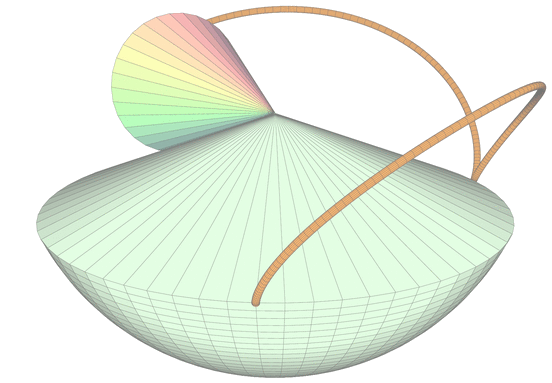
\includegraphics[width=4cm]{logo.png}}
\mail{}
\webpage{}
\collaboration{“我要明确告诉大家,中国开放的大门不会关闭,只会越开越大!'' \\ By -- 习~近~平}

\bibliography{biblio.bib}
\usefonttheme{serif}
\usepackage{csquotes}
\setbeamercolor{structure}{bg=black!5}




\begin{document}

\maketitle
\sepframe[title={目\quad \quad 录}]
\section{中国开放的决心和行动}
\sepframe[title={中国开放的决心和行动}, image ={
\includegraphics[width =4cm]{figures/党章.png}}]

\subsection{中国开放的决心}
\begin{frame}[fragile]{中国开放的决心}
    \begin{itemize}[<+-|alert@+>]
    \item 中国开放的大门只会越开越大,我们必须主动创新、扩大开放。对外开放是我国的基本国策。中国42年来有目共睹的经济社会发展成就,与开放是密不可分的。开放推动了改革,开放促进了发展。中国将进一步深化改革,扩大开放。这既符合中国自身发展利益,也有利于维护自由贸易,促进全球化健康发展。中国作为最大的发展中国家,实现现代化还有很长的路要走。中国对外开放的大门将越开越大,我们愿意借鉴国外先进技术和管理经验,扩大产品、知识、技术、服务等领域合作,不断放宽外商投资市场准入,提供更加法治化、便利化的营商环境。
    \item 中国开放的大门只会越开越大,我们必须主动创新、扩大开放。对外开放是我国的基本国策。中国42年来有目共睹的经济社会发展成就,与开放是密不可分的。开放推动了改革,开放促进了发展。中国将进一步深化改革,扩大开放。这既符合中国自身发展利益,也有利于维护自由贸易,促进全球化健康发展。中国作为最大的发展中国家,实现现代化还有很长的路要走。中国对外开放的大门将越开越大,我们愿意借鉴国外先进技术和管理经验,扩大产品、知识、技术、服务等领域合作,不断放宽外商投资市场准入,提供更加法治化、便利化的营商环境。
    \end{itemize}
\end{frame}

\begin{frame}
    \begin{itemize}[<+-|alert@+>]
        \item 中国开放的大门只会越开越大,我们必须笃定信心、坚定决心。诚如发展以后的问题并不比不发展的问题少,扩大开放也不会一帆风顺、万事大吉。然而,我们也不能因此前怕狼、后怕虎,既然开放的大门越开越大,就要任凭风浪起、稳坐钓鱼台,以一往无前的信心决心,锚定目标、选准路径,在开放融通的世界格局;中走得更好、走得更远,真正唱响中国声音、贡献中国力量。
        \item 开放带来进步,封闭必然落后。中国开放的大门不会关闭,只会越开越大。“一个国家、一个民族要振兴,就必须在历史前进的逻辑中前进,在时代发展的潮流中发展”习近平总书记站在人类历史发展进程的高度提出的思想,体现了中国致力于为世界和平与发展作出更大贡献的崇高目标;中国和平发展、国门越开越大的战略,体现了中国将自身发展与世界发展相统一的全球视野、世界胸怀和大国担当。
    \end{itemize}
\end{frame}
\subsection{中国开放的行动}

\begin{frame}[fragile]{中国拥抱开放的行动一直在}
\begin{itemize}[<+-|alert@+>]
    \item “一带一路”建设是我国扩大对外开放的重大举措,要一步一个脚印推进实施,建设好这条开放之路、合作之路、希望之路、共赢之路。共建“一带一路”是参与全球开放合作、改善全球经济治理体系、促进全球共同发展繁荣、推动构建人类命运共同体的中国方案。经过夯基垒台、立柱架梁的5年,正在向落地生根、持久发展的阶段迈进。现在的重点是在保持健康良性发展势头的基础上向高质量发展转变。建设“一带一路”,不打地缘博弈小算盘,不搞封闭排他小圈子,不做凌驾于人的强买强卖,而是努力打造成顺应经济全球化潮流的最广泛国际合作平台,打造成推动构建人类命运共同体的实践平台,以切实的行动推进构建人类命运共同体。
    \item 党的十八大以来,我国顺应国内消费升级趋势,采取更加积极有效的政策措施,持续释放国内市场潜力,扩大进口空间。从2018年开始,我国每年举办中国国际进口博览会。一个个参展台前人潮涌动,一场场交易洽谈密集开展,一个个签约合作接连达成,我国以更多务实行动和举措,同世界分享发展红利,助力经济全球化的时代浪潮奔腾不息、永远向前。
\end{itemize}
    

\end{frame}

\begin{frame}
\pause[1] \begin{quotation}[习近平]
    党的十八大以来,我国顺应国内消费升级趋势,采取更加积极有效的政策措施,持续释放国内市场潜力,扩大进口空间。从2018年开始,我国每年举办中国国际进口博览会。一个个参展台前人潮涌动,一场场交易洽谈密集开展,一个个签约合作接连达成,我国以更多务实行动和举措,同世界分享发展红利,助力经济全球化的时代浪潮奔腾不息、永远向前。
\end{quotation}
    

\end{frame}
\section{中国开放的范例}
\subsection{中国开放的范例-特斯拉进入中国}
\begin{frame}[fragile]{范例1-特斯拉进入中国}
\pause[1]\begin{alertblock}{特斯拉进入中国的现实意义}
    当年开工、当年竣工、当年投产、当年上市……在特斯拉上海“超级工厂”开工建设一周年之际,“中国版”Model Y生产项目宣布启动,马斯克专程飞抵上海向首批社会车主交付国产Model 3。而在此前,特斯拉已向员工交付了15辆蓝色和灰色的国产特斯拉Model 3。

    今天的世界,究竟是需要开放合作、互联互通,还是需要关上大门、贸易保护,包括特斯拉在内的各大企业正在“用脚投票”。某种意义上,马斯克口中的感谢,不仅是对“中国速度”的无限感慨,更是对中国开放发展理念的感同身受。“全球来商”的盛景背后,正是中国市场所蕴含的强大势能。数据显示,自2008年以来,中国利用外资一直居全球前三位,连续25年居发展中国家首位,利用外资的结构不断优化。2019年1-9月份,中国利用外资同比增长2.9\%,而特斯拉,作为第一家全外资在华独立投资的车企,更带有某种标志性。“投资环境就像空气,空气清新才能吸引更多外资。”国际社会投出的信任票,就是对中国持续优化营商环境务实举措的最大赞许。
\end{alertblock}

\end{frame}
\subsection{中国开放的范例-深圳的开放历程}
\begin{frame}[fragile]{范例2-深圳的开放历程}
  \begin{columns}
  \begin{column}{.5\linewidth}
  \includegraphics<1>[width=.9\linewidth]{figures/改革开放初期.jpg}
  \includegraphics<2>[width=.6\linewidth]{figures/深圳.jpeg}
  \includegraphics<3>[width=.6\linewidth]{figures/深圳2.jpeg}
  \includegraphics<4>[width=.6\linewidth]{figures/深圳3.jpeg}
  \includegraphics<5>[width=.6\linewidth]{figures/深圳4.jpeg}
  \includegraphics<6>[width=.6\linewidth]{figures/深圳5.jpeg}
  \includegraphics<7>[width=.6\linewidth]{figures/深圳6.jpeg}
  \includegraphics<8>[width=.6\linewidth]{figures/深圳7.jpeg}
  \includegraphics<9>[width=.6\linewidth]{figures/厦门.jpeg}
  \includegraphics<10>[width=.6\linewidth]{figures/汕头1.jpeg}
  \end{column}

  \begin{column}{.5\linewidth}
  \setbeamercolor{alerted text}{fg=blue}
  \begin{itemize}
  \item<1-|alert@1> 改革开放初期历史
  \item<2-|alert@2-4> 改革开放以来的深圳对比图
  \item<5-|alert@5-7> 改革开放以来的珠海对比图
  \item<8-|alert@8-9> 改革开放以来的厦门对比图
  \item<10-|alert@10> 改革开放以来的汕头对比图
  \end{itemize}
  \end{column}
  \end{columns}
\end{frame}

\thanksframe{谢谢大家的聆听,请批评指正!}
























\end{document}